\documentclass{beamer}
\usepackage{apacite}
\usepackage{caption}
\usepackage[font=small, labelfont=bf]{subcaption}
\usepackage{textpos}
\usetheme{Darmstadt}
\usepackage{graphicx}
\usepackage{float}
%packages for definitions%%%%%%%%%%%%%%
\usepackage{blindtext}
\usepackage{scrextend}
\addtokomafont{labelinglabel}{\sffamily}
%%%%%%%%%%%%%%%%%%%%%%%%%%%%%%%%%%%%%%%
\AtBeginSection[]{
    \begin{frame}
    \vfill
    \centering
    \begin{beamercolorbox}[sep=8pt,center,shadow=true,rounded=true]{title}
        \usebeamerfont{title}\insertsectionhead\par%
    \end{beamercolorbox}
    \vfill
    \end{frame}
}
\title{Garaphlet Analysis for HiC data}
\author{Behnam Rasoolian}
\institute{Auburn University}
\definecolor{auburn_orange}{RGB}{221, 85, 12}
\definecolor{auburn_blue}{RGB}{3, 36, 77}
\date{}
\begin{document}
\frame{\titlepage}
%\addtobeamertemplate{frametitle}{}{%
%    \begin{textblock*}{100mm}(.8\textwidth,-1.65cm)
%        
\includegraphics[height=1.65cm,width=3cm]{figures/auburn_logo.jpeg}
%    \end{textblock*}}
\section{Biological Background}
\begin{frame}[t]
    \frametitle{Purpose of this research}
    \framesubtitle{Introduction}
    \begin{columns}
        \begin{column}{.5\textwidth}
            \begin{itemize}
                \item In this research we plan to find dissimilarities 
                    between normal cells and cancerous cells.
                \item Ideally, it is desirable to compare \textbf{3D confomation}
                    of genomes in order to make such comparisons.
            \end{itemize}
        \end{column}
        \begin{column}[c]{.5\textwidth}
            \begin{figure}
                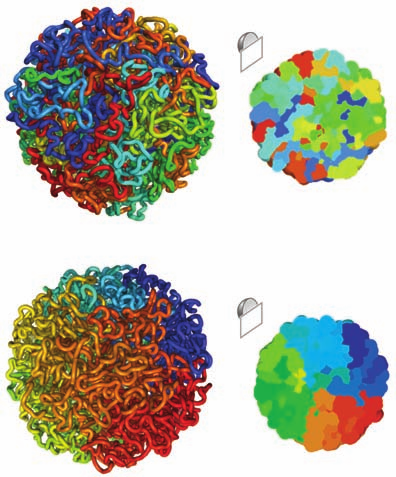
\includegraphics[width=.6\textwidth]{figures/chromosome_3d_structure.png}
                \caption*{ \cite{lieberman2009comprehensive}}
            \end{figure}
        \end{column}
    \end{columns}
\end{frame}

\begin{frame}
    \frametitle{Purpose of this research}
    \framesubtitle{Challenges}
        \begin{columns}
            \begin{column}[c]{.6\textwidth}
                \begin{itemize}
                        \item We still don't have enough information  
                            regarding the exact configuration
                        of a genome inside nucleus.
                        \item However, we can map interactions  in an
                        \textit{HiC contact map} ($C$).
                    \item Rows and columns signify genome fragments.
                    \item $C_{ij} = $ Number/strength of interactions detected between
                        fragment $i$ and $j$.
                \end{itemize}                                                                                 
            \end{column}
            \begin{column}{.4\textwidth}
                \begin{figure}
                    \centering
                    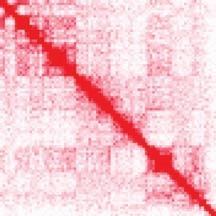
\includegraphics[width=\textwidth]{figures/original_contact_map_chr14.png}
                    \caption*{ \cite{lieberman2009comprehensive}}
                \end{figure}
            \end{column}
        \end{columns}
\end{frame}  
\begin{frame}
    \frametitle{Preliminaries}
    \framesubtitle{What is 3D conformation?}
    If you unfold the DNA inside one of your cells, it would measure
    2 meters end to end. How is it folded up withing a nucleus which
    is only 6 micorns wide?
    \begin{figure}
        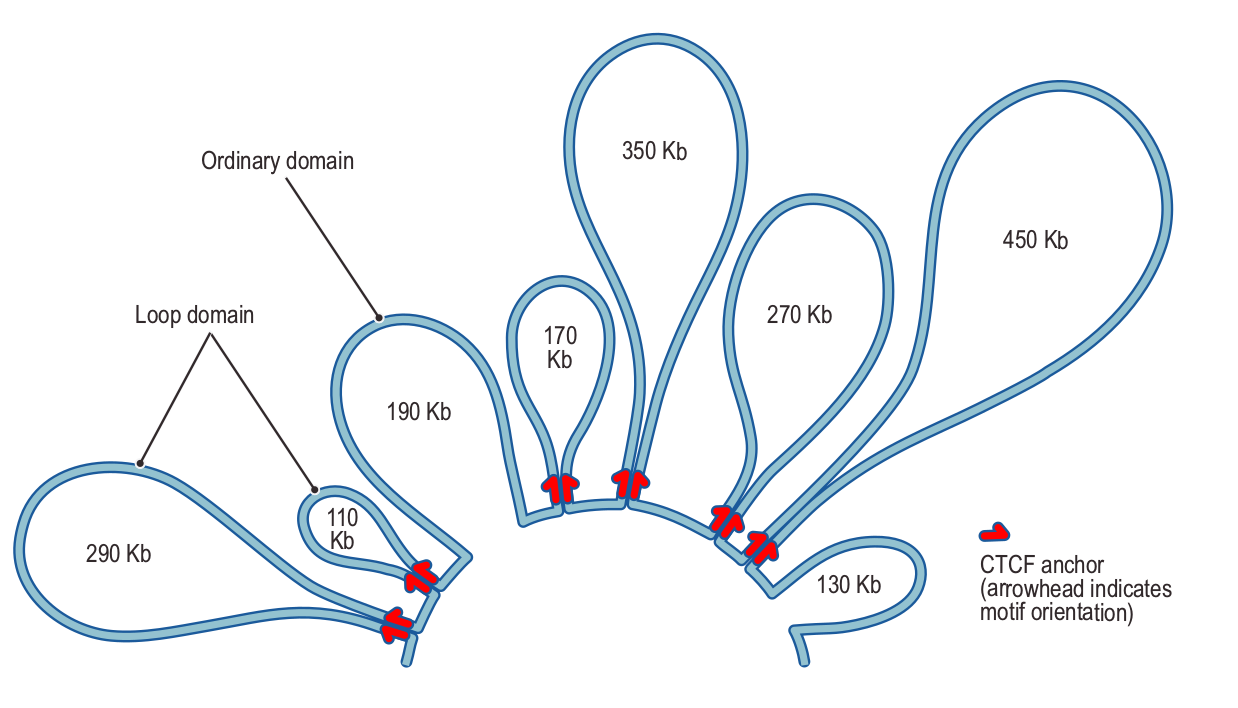
\includegraphics[width=.7\textwidth]{figures/loops.png}
        \caption*{ \cite{rao20143d}}
    \end{figure}
\end{frame}
\begin{frame}
    \frametitle{Preliminaries}
    \framesubtitle{Terminology \cite{wang2013properties}}
    \begin{columns}
        \begin{column}{1.15\textwidth}
     \fontsize{10}{10}\selectfont{
         \begin{itemize}
             \item \textbf{Nucleotide}:  The monomer units that comprise DNAs. There
        are 4 types of nucleotides: (C, G, A, and T)

        \item \textbf{Base}: Each pair of nucleotides in the DNA are called
        a base.
        \\A kilo-base resolution is a resolution that
        corresponds to 1000 pairs of nucleotides in DNA.

        \item \textbf{Nucleosome}: A basic unit 
        consisting of 145-147 bases wrapped around a
        protein complex. 

        \item \textbf{Chromatin Fiber}: Tens of nucleosomes are
        further collapsed into a larger dense structural unit
        of several kilobase (Kb) pairs.

        \item \textbf{Locus}: Multiple chromatin fibers form a large module of megabase pairs 
            (Mb) DNA, which may be referred to as \textit{domains, globules, gene
                 loci, or chromatin clusters} in different contexts.

        \item \textbf{Chromosome}: A number of loci then fold into a large
        independent physical structure, chromosome. 
         \end{itemize} }
        \end{column}
    \end{columns}
\end{frame}
\begin{frame}
    \frametitle{HiC Method}
    \framesubtitle{Procedure}
    \begin{columns}
        \begin{column}{1.1\textwidth}
            \begin{enumerate}
                \item Freeze the DNA in place.
                \item Cut the genome in tiny pieces.
                    Mark the ends using Biotin, and glue them together into
                    diffused pieces of DNA. These diffused pieces is made
                    up of two bits of the genome that are spatial neighbors.
                \item Using DNA sequencing, the two parts of the 
                    diffused DNA are identified and a dataset is created
                    where each cell corresponds to a pair.
            \end{enumerate}
        \end{column}
    \end{columns}
\end{frame}
\begin{frame}
    \frametitle{HiC Method}
    \framesubtitle{Illustration}
    \begin{figure}
        \centering
        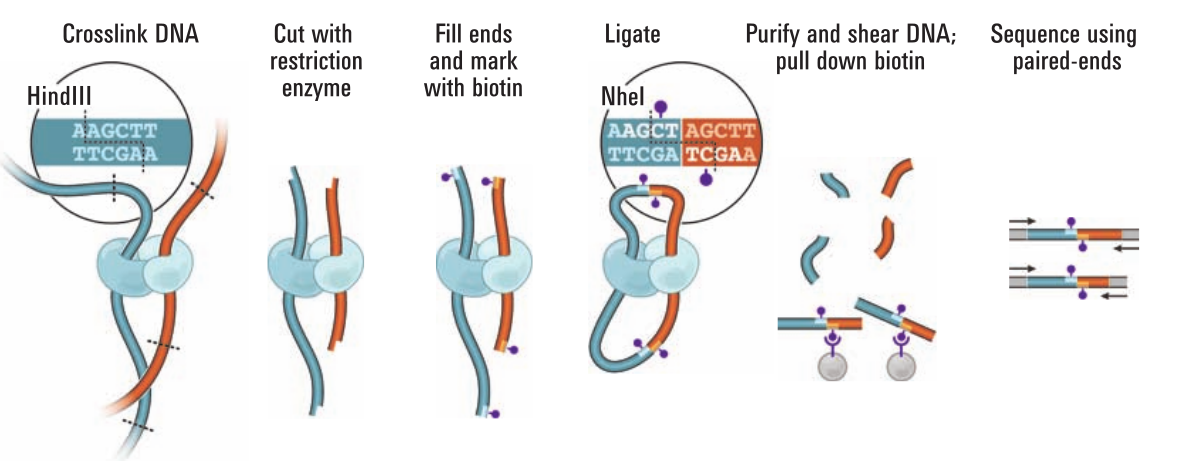
\includegraphics[width=1.1\textwidth]{figures/hic_process.png}
        \caption*{ \cite{lieberman2009comprehensive}}
    \end{figure}
\end{frame}

\begin{frame}
    \frametitle{HiC Method}
    \framesubtitle{Contact Maps}
    \begin{columns}
        \begin{column}{.5\textwidth}
            \begin{itemize}
                \item The whole genome is then divided into sections of certain length (i.e. 500kB or 1MB)
                    and interactions are aggregated over them.
                \item Contact maps can be used to develop both inter- and 
                    intra-chromosomal interaction matrices.

            \end{itemize}
        \end{column}
        \begin{column}{.5\textwidth}
            \begin{figure}
                \centering
                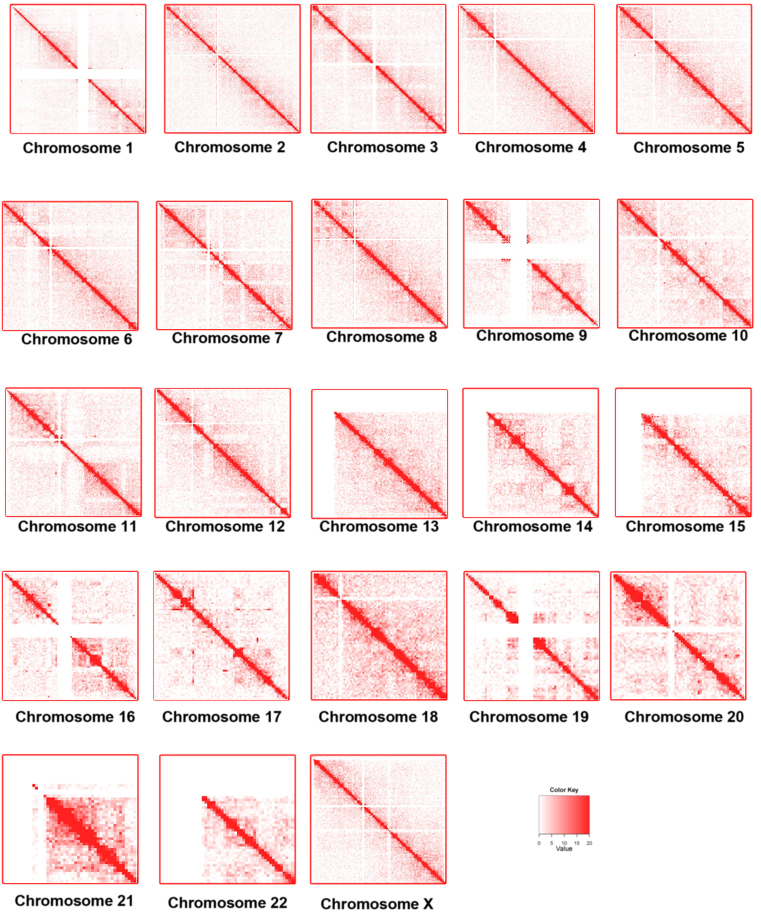
\includegraphics[width=.9\textwidth]{figures/normal-b-cell-all-heatmaps.jpeg}
                \caption*{\cite{wang2013properties}}
            \end{figure}
        \end{column}
    \end{columns}
\end{frame}
\section{Strategies}
\begin{frame}
    \frametitle{Graphlets}
    \framesubtitle{Definitions}
    Graphlet comparison, introduced by \citeA{prvzulj2007biological},
    is a novel method used to compare large networks in order to
    find local similarities in them.
    \begin{itemize}
        \item \textbf{Fragment:} A connected subgraph.
        \item \textbf{Motifs:} Fragments that occur with a frequency much higher than
            that occuring in a randomly generated graph.
        \item \textbf{Graphlets:} An arbitrary, induced fragment.
        An edge is the only two-node graphlet.
        \item \textbf{Induced graphs:} Given a graph $G(V, E)$ and $S \subseteq V$,
            then $G'(S, E')$
            is a graphlet iff $E' = \{(u, v) | u, v \in V \text{ and } 
            (u, v) \in E \rightarrow (u, v) \in E'\}$
        \item \textbf{Orbits:} Set of all nodes in a graphlet that can be
            swapped with each other while not changing the graph.
    \end{itemize}
\end{frame}

\begin{frame}
    \frametitle{Graphlets}
    \begin{figure}
        \centering
        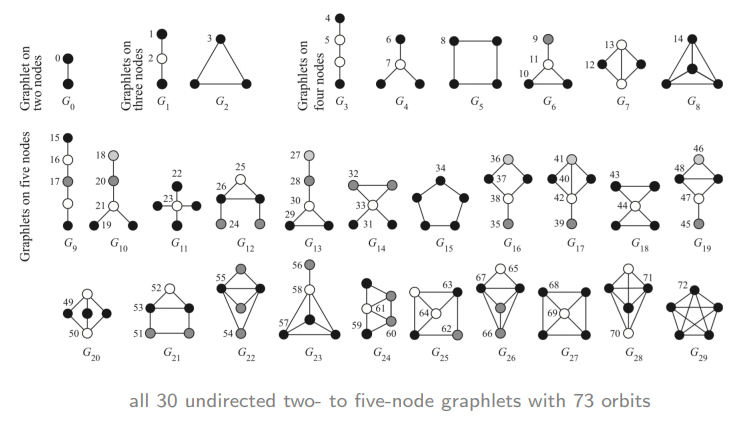
\includegraphics[scale=.4]{graphlets.png}
        \caption*{All 30 undirected two- to five-node
        graphlets with 73 orbits \cite{prvzulj2007biological}}
    \end{figure}
\end{frame}
\begin{frame}
    \frametitle{Graphlets}
    \framesubtitle{Applications}
    \textbf{\citeA{milenkoviae2008uncovering}:}

    \textit{Signature vector:} A 73-dimensional vector
    $\mathbf{s}^T
    = [s_0, s_2, ..., s_{72}]$ where $s_i$ denotes the number of nodes in
    the network that are part of an orbit $i$.
    
    \textit{Important Result}: Proteins with similar surroundings perform
    similar functions.
    \begin{figure}[H]
        \centering
        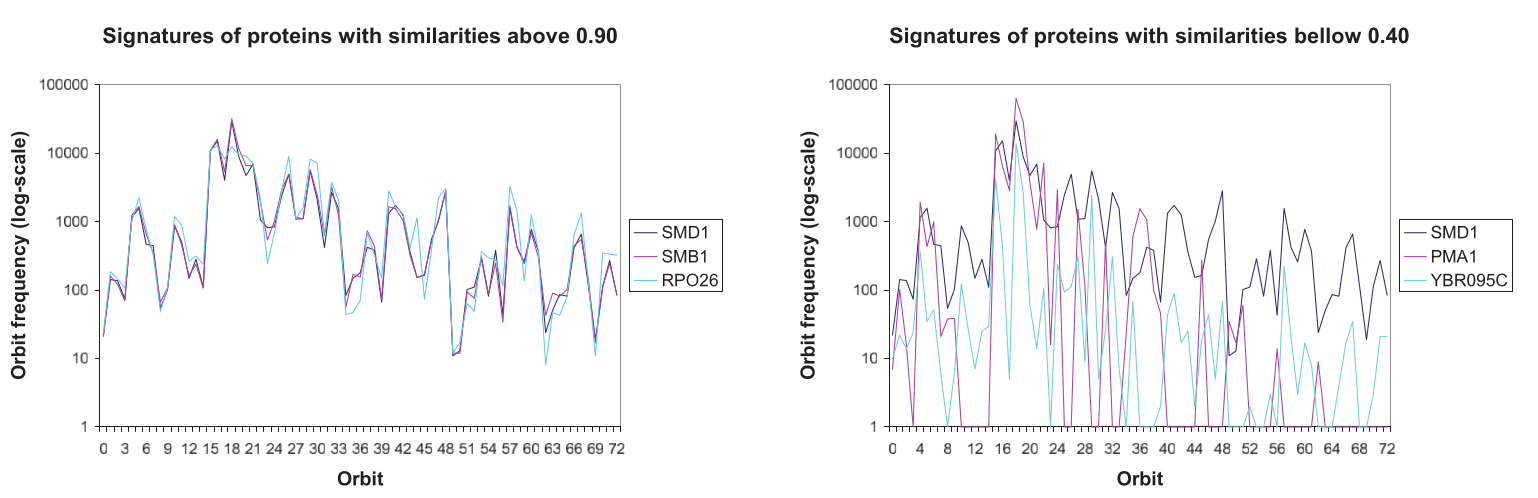
\includegraphics[width=\textwidth]{figures/signature-comparison.png}
        \caption*{\cite{milenkoviae2008uncovering}}
    \end{figure}
\end{frame}
\begin{frame}
    \frametitle{Introduction}
    \textbf{\citeA{milenkovic2010cancer}}: 

    Investigate cancer-causing genes to find similarities in their signatures. 
    \begin{enumerate}
        \item Cluster the genes based on \textit{signature similarity} criteria.
            Some clusters contain a lot of cancerous genes.
        
        \item Predict the cancer-relatedness of a protein $i$ using
            an enrichment criteria $\frac{k}{|C_i|}$ \\
            \begin{itemize}
                \item $C_i$ : the cluster where protein $i$ belongs\\
                \item $k$ : the number of cancer-causing proteins in $C_i$ \\
                \item $|C_i|$ : the size of $C_i$
            \end{itemize}
    \end{enumerate}
\end{frame}
\begin{frame}
    \frametitle{Graphlets}
    \framesubtitle{Challenges}
    \begin{enumerate}
        \item HiC contact maps are noisy. How do we de-noise them?
        \item Current applications of graphlets were on unweighted
            graphs, while HiC contact maps are weighted.
    \end{enumerate}
\end{frame}

\begin{frame}
    \frametitle{Balanced Network Deconvolution}
    \framesubtitle{Introduction}
    Proposed by \citeA{feizi2013network}, Balanced Network Deconvolution, is 
    a method that can be used to remove \textit{indirect effects} from a graph.
    \begin{figure}
        \centering
        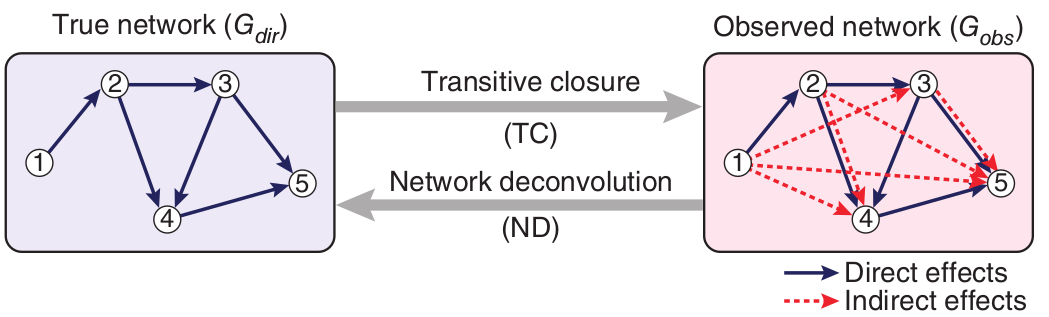
\includegraphics[width=\textwidth]{figures/nd.png}
        \caption*{ \cite{feizi2013network}}
    \end{figure}
\end{frame}
\begin{frame}
    \frametitle{Balanced Network Deconvolution}
    \framesubtitle{Details}
    They assume that:
    \begin{equation}
        \label{indirect_effects}
        G_{obs} = G_{dir} + G_{dir}^2 + G_{dir} + ...
    \end{equation}
    They assume also that both $G_{obs}$ and $G_{dir}$ can be 
    eigen-decomposed and they have the same eigen-vectors:
    \begin{equation}
        G_{dir} = X \Sigma_{dir} X^T
    \end{equation}
    \begin{equation}
        G_{obs} = X \Sigma_{obs} X^T
    \end{equation}
    \begin{equation}
        G_{obs} = X \Sigma_{obs} X^T = X ( \Sigma_{dir} + \Sigma_{dir}^2 + ...) X^T
    \end{equation}
\end{frame}
\begin{frame}
    \frametitle{Balanced Network Deconvolution}
    \framesubtitle{Details}
    They also assume that eigen-values of the direct network are all
    between -1 and 1, i.e. 
    \begin{equation}
        -1 < \lambda^{dir}_i < 1 \quad \forall 1 \le i \le n
    \end{equation}
    \begin{equation}
        \Sigma_{obs} = \Sigma_{dir} + \Sigma_{dir}^2 + ...
    \end{equation}
    \begin{equation}
        \lambda_i^{obs} = \sum_{j=1}^{\infty} \lambda^{dir}_{ij} \quad\quad \forall i = 1 ... n
    \end{equation}
    \begin{equation}
        \lambda_i^{obs} = \frac{\lambda_i^{dir}}{1 - \lambda_i^{dir}}
    \end{equation}
    \begin{equation}
       \lambda_i^{dir} = \frac{\lambda_i^{obs}}{1 + \lambda_i^{obs}} 
    \end{equation}
\end{frame}
\begin{frame}
    \frametitle{Statistical Parametric Network (SPN)}
    Developed by \citeA{ginestet2011statistical}.
    \begin{figure}
        \centering
        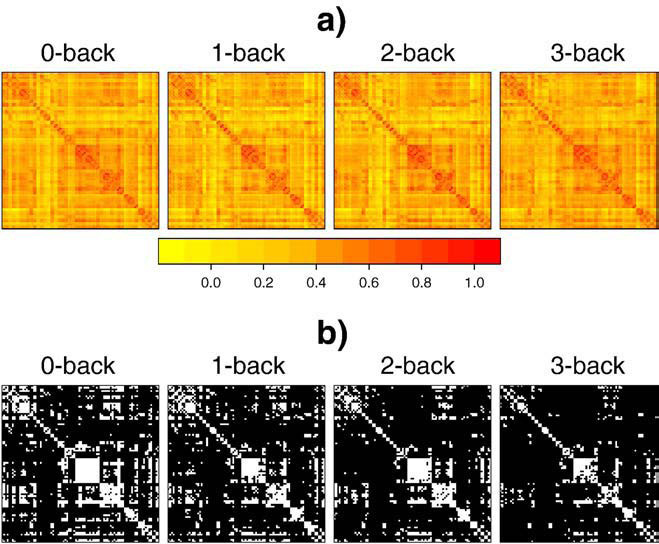
\includegraphics[width=.5\textwidth]{figures/thresholded_adjacency.png}
        \caption*{An study of neuron connectivity
            networks among 43 subjects for 4 different memory tasks 
            (0-back, 1-back, 2-back and 3-back), and the
            resulting thresholded networks \cite{ginestet2011statistical}}
        \label{fig:thresholded_adjacency}
    \end{figure}
\end{frame}
\section{Results Thus Far}
\begin{frame}
    \frametitle{Histogram of frequencies in HiC}
    \begin{figure}[H]
        \centering
        \begin{subfigure}[b]{.45\textwidth} 
            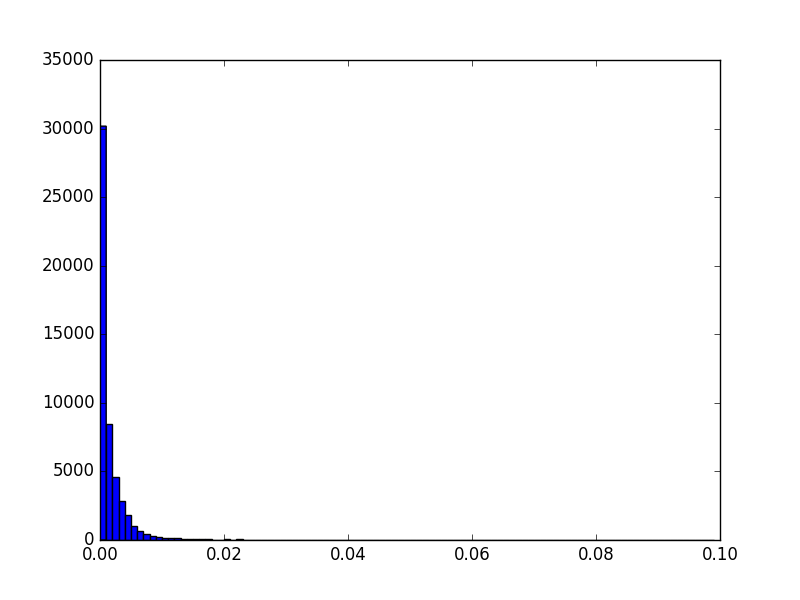
\includegraphics[width=\textwidth]{figures/hist01.png}
            \caption{Interval $[0, 0.1]$}
            \label{fig:hist01}
        \end{subfigure}
        \begin{subfigure}[b]{.45\textwidth}
            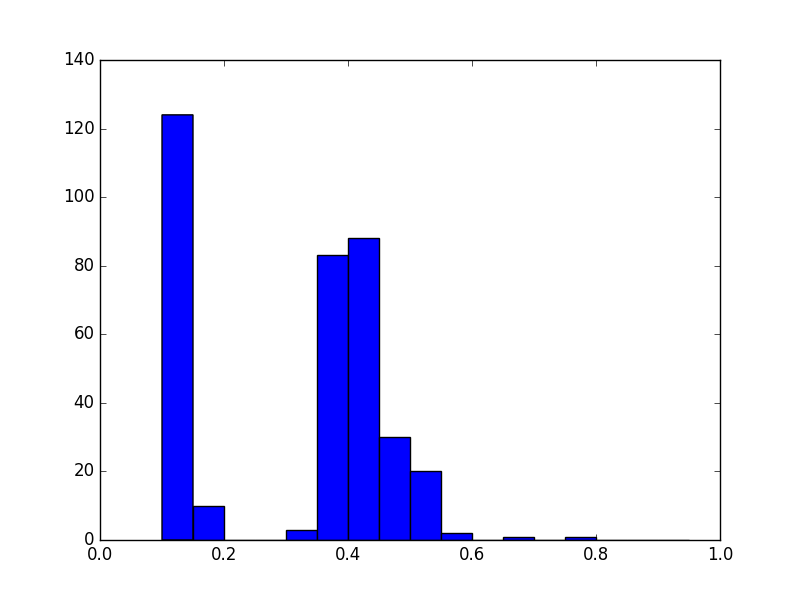
\includegraphics[width=\textwidth]{figures/hist02.png}
            \caption{Interval $[0.1, 1]$}
            \label{fig:hist02}
        \end{subfigure}
        \caption{\ref{fig:hist01} is a histogram of intensities from
        chromosome 1 
        As can be seen, the two histograms are orders of magnitude
        different in terms of frequency.}
        \label{fig:hists}
    \end{figure}
\end{frame}
\begin{frame}
    \frametitle{Histogram of logarithm}
    \begin{figure}[H]
        \centering
        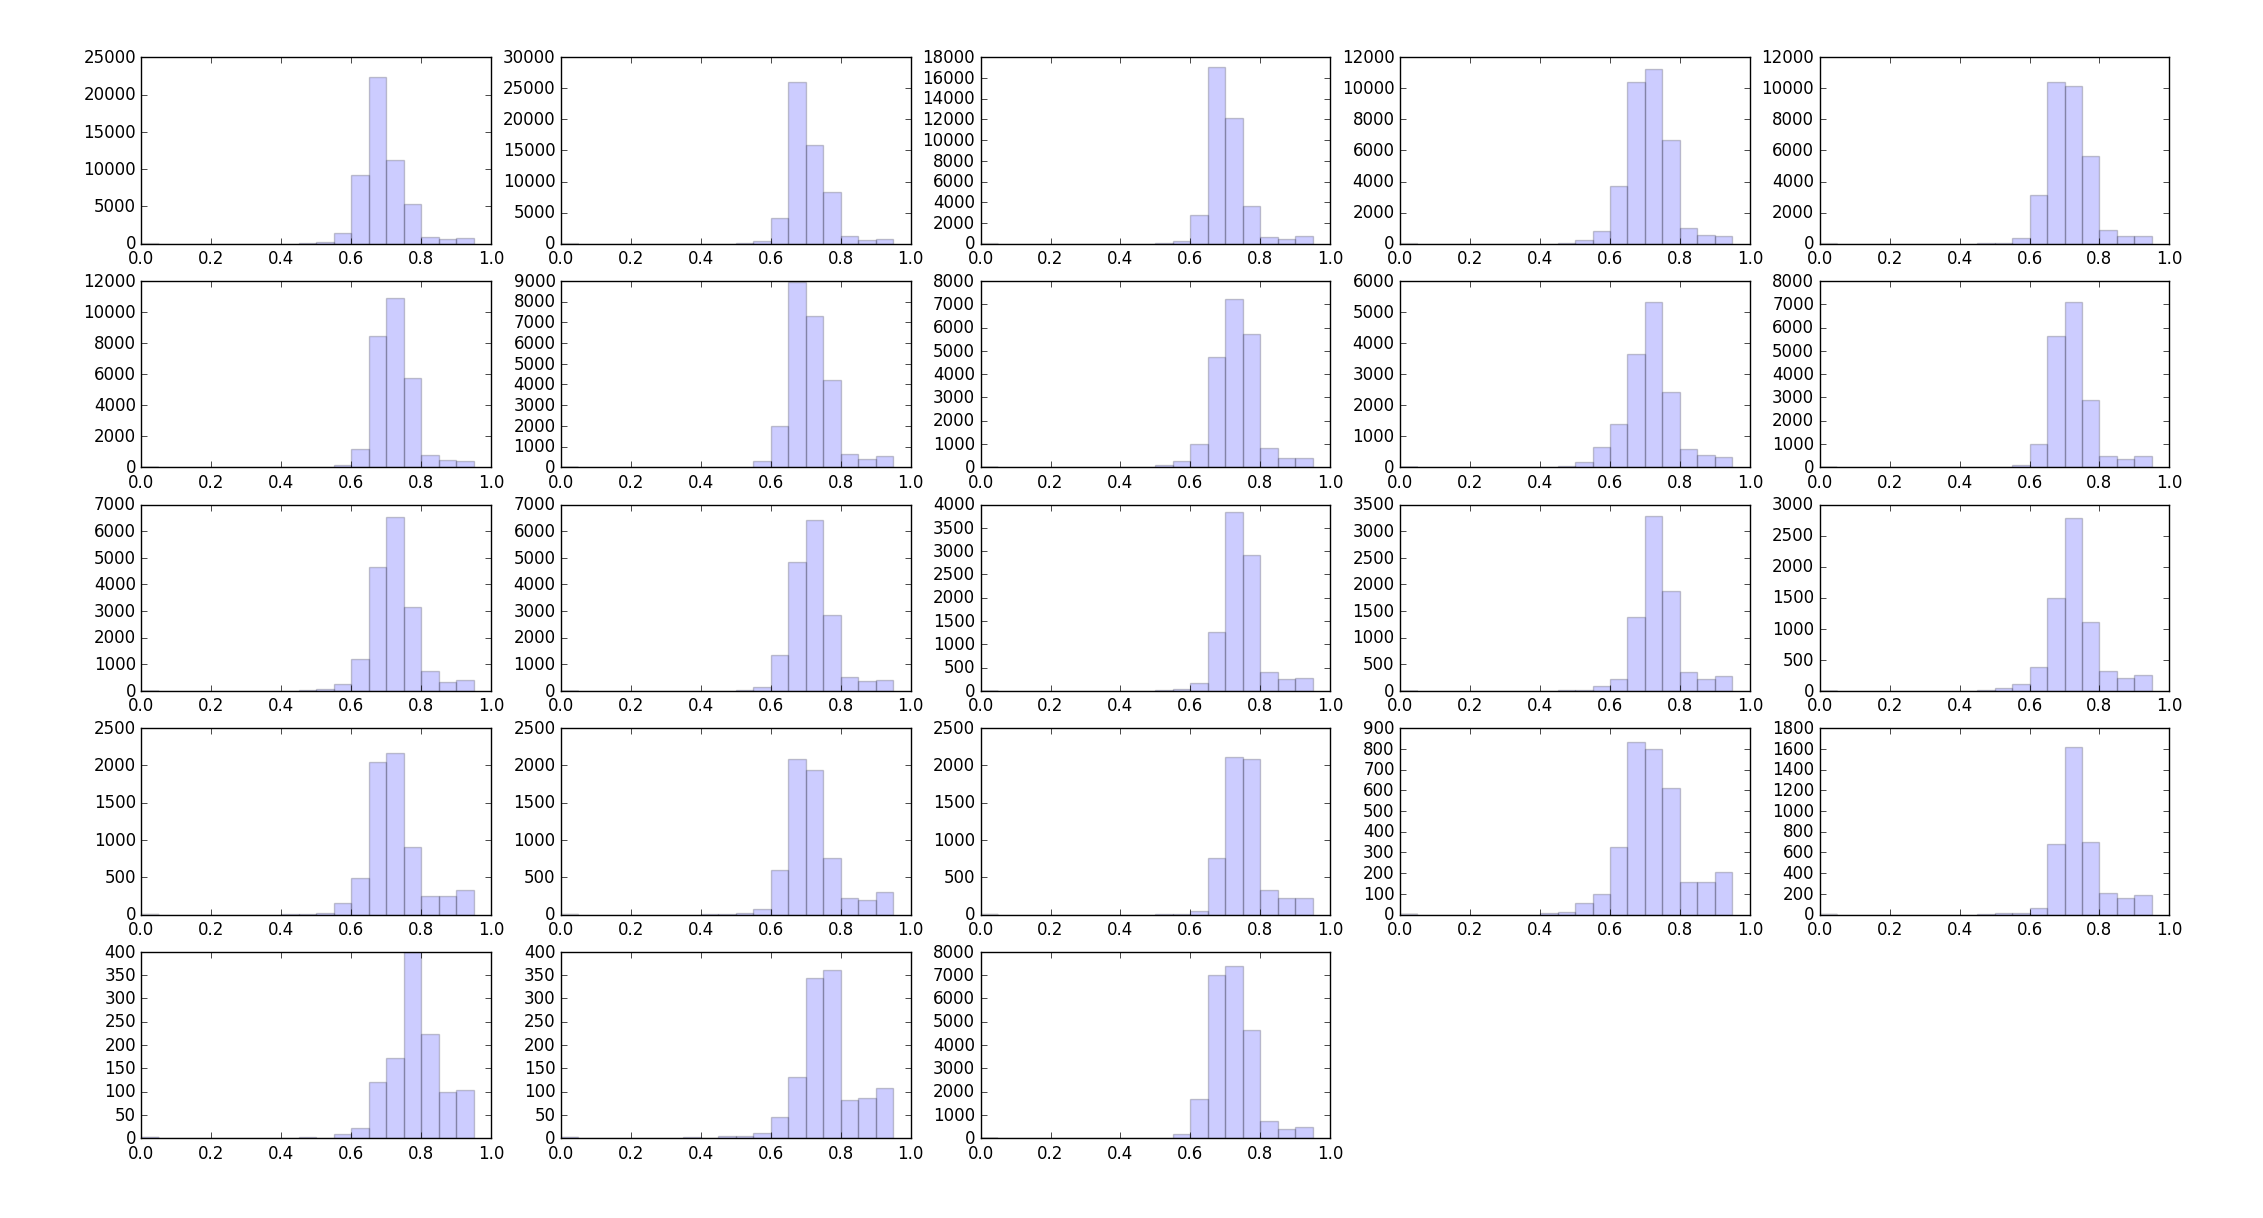
\includegraphics[width=1.05\textwidth]{figures/pyr_hist_1mb.png}
        \caption*{}
        \label{fig:pyr_hist_1mb}
    \end{figure}
\end{frame}
\begin{frame}
    \frametitle{Different Normalization methods}
    \begin{figure}[H]
        \centering
        \begin{subfigure}[b]{.25\textwidth}
            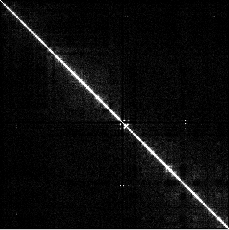
\includegraphics[width=\textwidth]{figures/original_cleaned.png}
            \caption{}
            \label{fig:original_cleaned}
        \end{subfigure}
        \begin{subfigure}[b]{.25\textwidth}
            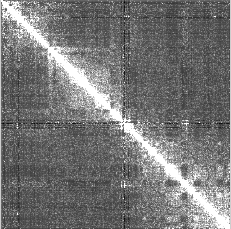
\includegraphics[width=\textwidth]{figures/pearson.png}
            \caption{}
            \label{fig:pearson}
        \end{subfigure}
        \begin{subfigure}[b]{.25\textwidth}
            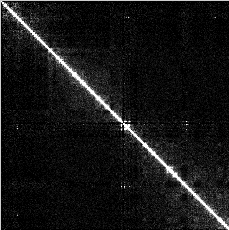
\includegraphics[width=\textwidth]{figures/scn.png}
            \caption{}
            \label{fig:scn}
        \end{subfigure}
        \begin{subfigure}[b]{.25\textwidth}
            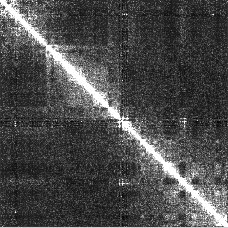
\includegraphics[width=\textwidth]{figures/scn+pearson.png}
            \caption{}
            \label{fig:scn+pearson}
        \end{subfigure}
        \begin{subfigure}[b]{.25\textwidth}
            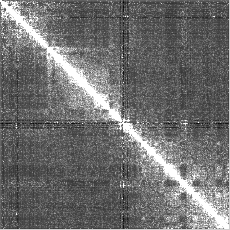
\includegraphics[width=\textwidth]{figures/pearson+scn.png}
            \caption{}
            \label{fig:pearson+scn}
        \end{subfigure}
        \begin{subfigure}[b]{.25\textwidth}
            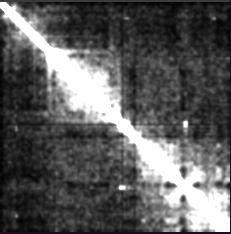
\includegraphics[width=\textwidth]{figures/pyr.png}
            \caption{}
            \label{fig:pyr}
        \end{subfigure}
        \caption*{}
        \label{fig:normalizations}
    \end{figure}
\end{frame}
\begin{frame}[allowframebreaks]
    \frametitle{References}
    \bibliographystyle{apacite}
    \bibliography{lit}
\end{frame}

\end{document}
